\documentclass[english,onecolumn]{elsarticle}
\usepackage[T1]{fontenc}
\usepackage[utf8]{inputenc}
\usepackage[a4paper]{geometry}
\geometry{verbose}
\usepackage{babel}
\usepackage{amsmath,amssymb,amsthm,bbm}
\usepackage{graphicx}
\usepackage{esint}
\usepackage[unicode=true]{hyperref}

\makeatletter

\usepackage{times}
%\usepackage{subfloat}
%\usepackage{subfig}
\usepackage{psfrag}
\usepackage{babel}

\def\d{\mathrm{d}}
\def\dmu{\mathrm{d}\mu}
\def\fD{\mathcal{D}}
\def\Rset{\mathbb{R}}
\def\X{\mathcal{X}}
\def\un{\mathbbm{1}}
\def\e{\operatorname{e}}
\def\W{\operatorname{W}}
\def\ext{\operatorname{ext}}
\def\sech{\operatorname{sech}}
\def\arsech{\operatorname{arsech}}
\def\argtanh{\operatorname{argtanh}}
%
\newcommand\Esp[1]{\mathbb{E}\left[ #1 \right]}

\newtheorem{definition}{Definition}
\newtheorem{proposition}{Proposition}

%%%
\makeatletter
\def\ps@pprintTitle{%
  \let\@oddhead\@empty
  \let\@evenhead\@empty
  \def\@oddfoot{\reset@font\hfil\thepage\hfil}
  \let\@evenfoot\@oddfoot
}
\makeatother

\makeatother

\begin{document}

\title{T'aurais pas une entropie?}


\author{by jfb \& co \date}
\begin{abstract}
  Where  we  show  that it  is  possible  to  derive  new entropies  yielding  a
  particular specified  maximum entropy distribution. There  are (probably) many
  errors  --I  hope  not  fundamental  but  is  is  possible;  (certainly  many)
  approximations,   typos,   maths   and   language   mistakes.Suggestions   and
  improvements will be much appreciated.
\end{abstract}
\maketitle

% -------------------- MaxEnt -------------------- %

\section{Maximum entropy distributions}
\label{sec:MaxEnt}

Let $f$ be a probability distribution  defined with respect to a general measure
$\mu$ on a set $\X$ and $\displaystyle  S[f] = - \int_\X f(x) \log f(x) \dmu(x)$
be  the Shannon  entropy of  $f$.   Subject to  $n$ moment  constraints such  as
$\Esp{T_i(x)} = t_i,  i = 1, \ldots,  n$ and to normalization, it  is well known
that the maximum entropy distribution lies within the exponential family
%
\[
f_X(x) = \exp\left( \sum_{i=1}^n \lambda_i T_i(x) + \lambda_0 \right).
\]
%
In order  to recover  known probability distributions  (that must belong  to the
exponential family), it is then sufficient  to specify a set of functions $T_i$.
This has been used by many authors.  For instance, the gamma distribution can be
viewed as a maximum entropy distribution  if one knows the moments $\Esp{X}$ and
$\Esp{\log(X)}$.  In  order to find  maximum entropy distributions  with simpler
constraints or distributions  outside of the exponential family,  it is possible
to  consider other  entropies,  which  is discussed  below.   This problem  find
interests in goodness-and-fit tests based on maximum entropy principle.


% -------------------- Max (h,phi)-Ent -------------------- %

\section{Maximum $(h,\phi)$-entropy distributions}
\label{sec:MaxPhiEnt}

% ---------- Definition & MaxEnt solutions

\subsection{Definition and maximum $(h,\phi)$-entropy solution}
\label{subsec:DefinitionPhiEnt}

\begin{definition}
  Let  $\phi:  \Omega  \subset  \Rset_+  \mapsto  \Rset$  be  a  strictly  convex
  differentiable function defined on a closed convex set $\Omega$.  Then, if $f$
  is  a probability  distribution  defined  with respect  to  a general  measure
  $\mu(x)$ on a set $\X$,
%
\begin{equation}
H_\phi[f] = - \int_\X \phi(f(x)) \dmu(x)
\label{eq:phi-entropy}
\end{equation}
%
is the $\phi$-entropy of $f$.
\label{def:phi_entropy}
\end{definition}
%
Since $\phi(x)$ is convex, then the entropy functional $H_\phi[f]$ is concave.
Also  note that  the composition  of a  concave function  with a  nondecreasing
concave function preserves concavity, and  that composition of a convex function
with a nonincreasing convex function yields a concave functional.

\begin{definition}%\cite{Sal93,Men97}
%
With the same assumption as in definition~\ref{def:phi_entropy},
%
\begin{equation}
H_{h,\phi}[f] = h\left( - \int_\X \phi(f(x)) \dmu(x) \right)
\label{eq:h-phi-entropy}
\end{equation}
%
is called $(h,\phi)$-entropy of $f$, where
%
\begin{itemize}
\item either $\phi$ is convex  and $h$ concave  nondecreasing,
\item or $\phi$ is concave and $h$ convex nonincreasing
\end{itemize}
\end{definition}
%
These  $(h,\phi)$-entropies  have   been  studied  in~\cite{Sal93,MenMor97}  for
instance. In  these works neither concavity  (resp.\ convexity) of  $h$, nor the
differentiability of $\phi$ are imposed.

A  useful  related  quantity  to  these  entropies  is  the  Bregman  divergence
associated with convex function $\phi$:
%
\begin{definition}
  With  the  same assumption  in  definition~\ref{def:phi_entropy}, the  Bregman
  divergence associated with $\phi$ defined  on a closed convex set $\Omega,$ is
  given by
  %
  \begin{equation}
    D_\phi(x_1,x_2) = \phi(x_1) - \phi(x_2) - \phi'(x_2) \left(x_1-x_2\right).
  \end{equation}
  %
  \label{def:Bregman}
\end{definition}
%
A direct consequence  of the strict convexity of $\phi$  is the nonnegativity of
the Bregman  divergence: $D_\phi(x_1,x_2)  \ge 0$ with  equality if and  only if
$x_1 = x_2$.

\

Consider the  problem of maximizing entropy  \eqref{eq:h-phi-entropy} subject to
constraints  on some  moments  $\Esp{T_i(X)}$. Without  loss  of generality,  we
consider in the sequel that $\phi$  is convex. Since $h$ is nondecreasing, it is
enough to look for the maximum of the $\phi$-entropy \eqref{eq:phi-entropy},
%
\begin{equation}
\begin{cases}
\max_f & \displaystyle - \int_\X \phi(f(x)) \dmu(x)\\[5mm]
%
\text{s.t. } & \displaystyle \int_\X f(x) \dmu(x) = 1\\[5mm]
%
\text{s.t. } & \Esp{T_i(X)} = t_i, \quad i = 1, \ldots, n
%
\end{cases}
\label{eq:MaxEnt}
\end{equation}
%
\begin{proposition}
  The   probability  distribution   $f_X$  solution   of  the   maximum  entropy
  problem~\eqref{eq:MaxEnt} satisfies the equation
%
\begin{equation}
\phi' \big( f_X(x;t) \big) = \lambda_0 + \sum_{i=1}^n \lambda_i \, T_i(x),
\label{eq:sol-h-phi}
\end{equation}
%
where  parameters  $\lambda_i$ are  such  that  the constraints  (normalization,
moments) are satisfied.
% $\Esp{T(X)} = t$.
\end{proposition}
%
\begin{proof}
%
  The maximization  problem being  concave, the solution  exists and  is unique.
  Equation~\eqref{eq:sol-h-phi}  results directly  from  the classical  Lagrange
  multipliers technique.

  An  alternative  derivation  of  the  result consists  in  checking  that  the
  distribution   \eqref{eq:sol-h-phi}   is   effectively   a   maximum   entropy
  distribution,  by showing  that $H_\phi[f]  > H_\phi[g]$  for  all probability
  distributions with given (fixed) moments $\Esp{T_i(X)}$. To this end, consider
  the  functional Bregman  divergence acting  on  functions defined  on a  common
  domain $\X$:
%
\[
\fD_\phi(f_1,f_2) = \int_\X \phi(f_1(x)) \dmu(x) - \int_\X \phi(f_2(x))
\dmu(x) - \int_\X \phi'(f_2(x)) \left( f_1(x) - f_2(x) \right) \dmu(x).
\]
%
From the nonnegativity  of the Bregman divergence this  functional divergence is
nonnegative as  well, and  zero if and  only if  $f_1 = f_2$  almost everywhere.
Define by
%
\[
C_t = \left\{ f: \X \mapsto \Rset_+: \:\: \int_\X f(x) \dmu(x) = 1, \:\:
\Esp{T_i(X)} = t_i, \: i = 1, \ldots, n \right\} 
\]
%
the set of all probability distributions defined on $\X$ with given moments $t =
(t_1 ,  \ldots , t_n)$.  Consider now  $f_X \in C_t$ such  that $\phi'(f_X(x)) =
\displaystyle  \lambda_0  + \sum_{i=1}^n  \lambda_i  \,  T_i(x)$  and any  given
function $f \in C_t$. Then
% 
\begin{eqnarray*}
\fD_\phi(f,f_X) & = & \int_\X \phi(f(x)) \dmu(x) - \int_\X \phi(f_X(x))
\dmu(x) - \int_\X \phi'(f_X(x)) \left( f(x) - f_X(x) \right) \dmu(x)\\[2mm]
%
& = & - H_\phi[f] + H_\phi[f_X] - \int_\X \left( \lambda_0 + \sum_{i=1}^n
\lambda_i \, T_i(x) \right) \left( f(x) - f_X(x) \right) \dmu(x)\\[2mm]
%
& = & H_\phi[f_X] - H_\phi[f]
\end{eqnarray*}
%
where we  used the fact that  $f$ and $f_X$ have  both probability distributions
with  the same moments  $\Esp{T_i(X)} =  t_i$.  By  nonnegativity of  the Bregman
functional divergence, we finally get that
%
\[
H_\phi[f_X] \ge H_\phi[f]
\]
%
for all distribution $f$ with the same  moments $t$ than $f_X$, with equality if and only
if $f = f_X$ almost everywhere.  In other words, this shows that $f_X$, solution
of \eqref{eq:sol-h-phi}, realizes the minimum of $H_\phi[f]$ over $C_t$.
\end{proof}


% ---------- New entropy functionals

\subsection{Defining new entropy functionals}
\label{subsec:NewPhiEnt}

Given  an entropy  functional, we  thus obtain  a maximum  entropy distribution.
There exists numerous  $(h,\phi)$-entropies in the literature. However  a few of
them lead to explicit forms for the maximum entropy distribution.  Therefore, it
is  of  high interest  to  look  for the  entropies  that  lead  to a  specified
distribution as a maximum entropy solution. As pointed out previously, this find
interests in goodness-and-fit  tests based in entropies: it  seems convenient to
realize  such  tests  using  the  entropy  such  that  the  distribution  tested
corresponds to its maximum entropy.

Since we will look for the  function $\phi$ for a given probability distribution
$f_X(x)$ we also see that the corresponding $\lambda$ parameters can be included
in the definition of the function.

Let us recall some implicit properties of $\phi(x)$.
%
\begin{itemize}
\item $\phi'(x)$ is defined on a domain that includes $f_X(\X)$;
%
\item  From the  strict convexity  property  of $\phi$,  necessarily $\phi'$  is
  increasing.
\end{itemize}
%
The identification  of a function  $\phi(x)$ such that  a given $f_X(x)$  is the
associated maximum  entropy distribution amounts  to solve \eqref{eq:sol-h-phi},
that is:
%
\begin{enumerate}
\item choose a set of functions $T_i(x)$, $i = 1, \ldots, n$,
%
\item find $\phi'$ satisfying  $\displaystyle \lambda_0 + \sum_{i=1}^n \lambda_i
  T_i(x) = \phi'(f_X(x))$,
%
\item integrate the result to get  $\displaystyle \phi(y) = \int \phi'(y) \d y +
  c$,  where $c$  is  an integration  constant.   The entropy  being defined  by
  $\displaystyle  H_\phi[f] = -  \int_\X \phi(f(x))  \dmu(x)$, the  constant $c$
  will usually be zero.
% 
\item Parameters  $\lambda_i$ may be chosen  case by case in  order to simplify
  the expression of $\phi$.
\end{enumerate}

Remind  that  $\phi'$  must  be increasing,  thus,  necessarily,  $\displaystyle
\sum_{i=1}^n  \lambda_i \,  T_i(x)$ and  $f_X(x)$ must  have the  same  sense of
variation.  Moreover, at a first glance, eq.~\eqref{eq:sol-h-phi} requires these
two  quantities to  share the  same symmetries.   Namely, if  for  two different
values $x_1, x_2  \in \X$ the distribution satisfies  $f_X(x_1) = f_X(x_2)$ then
$\displaystyle \sum_{i=1}^n  \lambda_i \,  T_i(x_1) = \sum_{i=1}^n  \lambda_i \,
T_i(x_2)$ (this does  mean that $T_i(x_1)$ and $T_i(x_2)$  must be equal). Thus,
eq.~\eqref{eq:sol-h-phi} rewrites
%
\begin{equation}
\phi'(y) = \lambda_0 + \sum_{i=1}^n \lambda_i \, T_i \! \left( f_X^{-1}(y)
\right),
\label{eq:derivative-phi}
\end{equation}
%
where $f_X^{-1}$ can  be multivalued; in such a  situation, $\phi'$ remains well
defined. Note again  that for given $T_i$ and $f_X$, the  solution is not unique
due to parameters $\lambda_i$, which can  be chosen finely so as to simplify the
expression of $\phi'$. Eq.~\eqref{eq:derivative-phi}  can then be integrated, at
least  formally, to  achieve $H_\phi$  (and  thus any  $H_{h,\phi}$ entropy  with
nondecreasing $h$).

For instance, for one moment constraint, if $\lambda_1$ is negative, then
%
\begin{itemize}
\item for $T_1(x) = x,$ $f_X(x)$ must be decreasing,
\item for $T_1(x) = x^2$ or $T_1(x) = |x|,$ $f_X(x)$ must be even and unimodal.
\end{itemize}


% -------------------- Multiform Ent -------------------- %

\section{Multiform entropies}
\label{sec:MultiformEnt}

Of  course,  the preceding  derivations  require  that \eqref{eq:sol-h-phi}  is
effectively solvable.   In addition, one has  also to choose  or design specific
$T_i(x)$ statistics, as well as the  parameters $\lambda_i$ so as to respect the
symmetries of  the problem.  In  the examples above,  we used $T_1(x) =  x$, and
thus $f_X$  must be  monotone.  Similarly  the choice $T_1(x)  = x^2$  or $|x|$
obviously lead to symmetrical densities as already mentioned.

For  nonsymmetrical  unimodal densities  for  instance,  the  situation is  more
involved.   For instance,  if  we take  $T_1(x) =  x$,  then, on  $\X =  \Rset$,
eq.~\eqref{eq:sol-h-phi} has  no solution.   Two ways of  making (at  least) are
possible and  can consist in considering multivalued  functions $\phi$, allowing
to ``asymetrize'' the problem: thus, either one can specify the constraints only
on well suited intervals in order to preserve the concavity of the hence defined
$\phi$-entropy, or to keep the constraint  over $\X$ be loosing the concavity of
the  entropy.  Let  us  now   investigate  more  precisely  these  two  possible
approaches.


% ---------- Concave multiform

\subsection{Concave entropy with partial moments constraints}
\label{subsec:ConcaveMultiPhiEnt}

Let  us consider
%
\begin{itemize}
\item a partition $(\X_1,\ldots,\X_k)$ of $\X$ and
\item  a multivalued  function $\phi$  with  $k$ branches  $\phi_l$, where  each
  branch is convex.
\end{itemize}
%
For  sake of  simplicity, consider  that the  $\phi_l$ are  defined on  the same
domain.  Let us then define a $\phi$-entropy as
%
\begin{equation}
H_\phi[f] = -  \int_\X \, \sum_{l=1}^k \phi_l(f(x)) \, \un_{\X_l}(x) \, \dmu(x)
\label{eq:multiform-phi}
\end{equation}
%
where  $\un_A$ denotes  the indicator  of set  $A$.  Clearly,  $H_\phi[f]$  is a
concave entropy.  Let  us consider now $l$ sets of $n_l  \ge 0$ constraints over
each domain, $\Esp{ T_{l,i}(X) \un_{\X_l}(X)} = t_{l,i}$, $l = 1, \ldots, k$ and
$i =  1, \ldots, n_l$ (by  convention, this set is  empty if $n_l  = 0$).  Thus,
with  the same  methodology than  in section~\ref{sec:MaxPhiEnt} (Lagrange  technique, a
posteriori verification via Bregman  functional divergences associated with each
$\phi_l$), we achieve the following result
%
\begin{proposition}
  The   probability  distribution   $f_X$  solution   of  the   maximum  entropy
  problem
%
  \begin{equation}
  \begin{cases}
  \max_f & H_\phi[f]\\[5mm]
  %
  \text{s.t. } & \displaystyle \int_\X f(x) \dmu(x) = 1\\[5mm]
  %
  \text{s.t. } & \Esp{  T_{l,i}(X)  \un_{\X_l}(X)} = t_{l,i},
  \quad l = 1, \ldots, k, \quad i = 1, \ldots, n_l
  %
  \end{cases}
  \label{eq:MaxEntMultiConcave}
  \end{equation}
  %
  satisfies the equation
  %
  \begin{equation}
  \sum_{l=1}^k \phi_l' \big( f_X(x) \big) \un_{\X_l}(x) = \lambda_0 +
  \sum_{l=1}^k \sum_{i=1}^{n_l} \lambda_{l,i} \, T_{l,i}(x)  \un_{\X_l}(x)
  \label{eq:sol-phi-multi-concave}
  \end{equation}
%
  where  $\lambda_0, \lambda_{l,i}$  are  such that  the  normalization and  the
  constraints are satisfied and  $\displaystyle \sum_{i=1}^0$ is empty (or zero)
  by convention.
\end{proposition}

Now, the  identification of a multivalued  function $\phi(x)$ such  that a given
$f_X(x)$ is  the associated  maximum entropy distribution  generalizes following
the steps
%
\begin{enumerate}
\item  define  a partition  $(\X_1,\ldots,\X_k)$  of  $\X$  such that  $f_X$  is
  monotonous in each $\X_l$,
%
\item choose $n_l$ sets of functions $T_{l,i}(x)$ defined over $\X_l$,
%
\item find each $\phi_l'$ satisfying $\displaystyle \lambda_0 + \sum_{i=1}^{n_l}
  \lambda_{l,i} T_{l,i}(x) = \phi_l'(f_X(x))$ for $x \in \X_l$
%
\item integrate the results to get $\displaystyle \phi_l(y) = \int \phi_l'(y) \d
  y$.
% 
\item Again, parameters  $\lambda_0$ and $\lambda_{l,i}$ may be  chosen case by
  case in order to simplify the expression of the $\phi_l$.
\end{enumerate}

Since   the   $\phi_l'$   must   be  increasing,   necessarily,   $\displaystyle
\sum_{i=1}^{n_l} \lambda_{l,i}  \, T_{l,i}(x)$ and  $f_X(x)$ must have  the same
sense of variation on $\X_l$, and thus
%
\begin{equation}
\phi_l'(y) = \lambda_0 + \sum_{i=1}^{n_l} \lambda_{l,i} \, T_{l,i} \! \left(
f_{X,l}^{-1}(y) \right)
\label{eq:derivative-phil-concave}
\end{equation}
%
where $f_{X,l}^{-1}$ is the inverse of distribution $f_X$ defined over $\X_l$.

\

An advantage of  this approach is that  it allows to view any  distribution as a
maximum  entropy distribution  subjected  to simple  contraints since,  although
defined  via  a multiform  entropic  functional  $\phi$,  the concavity  of  the
$\phi$-entropy is preserved. Moreover,  the classical case is naturally included
in this extension.

The  major drawback  of this  approach is  that in  general constraints  must be
specified on  subsets $\X_l$ and not on  the whole domain of  definition $\X$ of
$f_X$. This is somewhat unnatural,  even if practically such partial moments can
be estimated by  thresholding properly the data.


% ---------- multiform and uniform moments

\subsection{Extremum entropy with uniform moments constraints}
\label{subsec:ExtremalPhiEnt}

An alternative to the previous approach  should be to preserve the definition of
constraints over the wole domain of  definition $\X$ of $f_X$, adapting then the
$\phi_l$ to each domain where $f_X$  is monotone. The consequence of this way of
making is that the convavity of the $\phi$-entropy we will derive is lost.

To  be  clearer,  let  us  again  consider  a  multiform  $\phi$-entropy  as  in
eq.~\eqref{eq:multiform-phi}, but  relaxing the concacity of  the $\phi_l$.  The
$\phi$-entropy is then not necessarily concave.  To distinguish this case to the
previous one, we will use the notation $\widetilde{\phi}_l$ instead of $\phi_l$.
%%
%\begin{equation}
%\widetilde{H}_\phi[f] = - \int_\X \, \sum_{l=1}^k \widetilde{\phi}_l(f(x)) \,
%\un_{\X_l}(x) \, \dmu(x)
%\label{eq:multiform-phi-nonconcave}
%\end{equation}
%
Thus, it  is no more possible to  interpret a distribution as  a maximal entropy
when this las  one turns to be not concave. However,  by the Lagrange technique,
we can  achieve an {\em  extremal entropy}  that can be  either a maximum,  or a
minimum,  or  a  saddle-point.  Let   us  denote  by  $\ext$  such  an  extremal
distribution, thus
%
\begin{proposition}
  The probability distribution $f_X$ solution of the extremal entropy problem
%
  \begin{equation}
  \begin{cases}
  \ext_f & H_\phi[f]\\[5mm]
  %
  \text{s.t. } & \displaystyle \int_\X f(x) \dmu(x) = 1\\[5mm]
  %
  \text{s.t. } & \Esp{T_i(X)} = t_i,  \quad i = 1, \ldots, n
  %
  \end{cases}
  \label{eq:ExtEntMulti}
  \end{equation}
  %
  satisfies the equation
  %
  \begin{equation}
  \sum_{l=1}^k \widetilde{\phi}_l' \big( f_X(x) \big) \un_{\X_l}(x) =
  \lambda_0 + \sum_{i=1}^n \lambda_i \, T_i(x)
  \label{eq:sol-phi-multi-notconcave}
  \end{equation}
%
  where  $\lambda_0,  \lambda_i$  are   such  that  the  normalization  and  the
  constraints are satisfied.
\end{proposition}

Since  $T_i(x)  =  \sum_l  T_i(x)  \un_{\X_l}(x)$, with  this  alternative,  the
identification of a multivalued function $\phi(x)$ such that a given $f_X(x)$ is
the  associated maximum  entropy  distribution generalizes  again following  the
steps
%
\begin{enumerate}
\item  define  a partition  $(\X_1,\ldots,\X_k)$  of  $\X$  such that  $f_X$  is
  monotonous in each $\X_l$,
%
\item choose $n$ functions $T_i(x)$ defined over $\X$,
%
\item  find  each $\widetilde{\phi}_l'$  satisfying  $\displaystyle \lambda_0  +
  \sum_{i=1}^n \lambda_i T_i(x) = \widetilde{\phi}_l'(f_X(x))$ for $x \in \X_l$
%
\item integrate  the results to get $\displaystyle  \widetilde{\phi}_l(y) = \int
  \widetilde{\phi}_l'(y) \d y$.
% 
\item Again, parameters  $\lambda_0$ and $\lambda_i$ may be  chosen case by case
  in order to simplify the  expression of the $\widetilde{\phi}_l$. Note however
  that the same $\lambda_i$ are linked to any $\widetilde{\phi}_l$.
\end{enumerate}

Now the  $\widetilde{\phi}_l'$ are  not imposed to  be increasing, but  they are
still under the form
%
\begin{equation}
\widetilde{\phi}_l'(y) = \lambda_0 + \sum_{i=1}^n \lambda_i \, T_i \! \left(
f_{X,l}^{-1}(y) \right)
\label{eq:derivative-phil-nonconcave}
\end{equation}
%
where $f_{X,l}^{-1}$  is the inverse  of distribution $f_X$ defined  over $\X_l$
and the same $\lambda_i$ for any $\widetilde{\phi}_l$. Note that
%
\begin{itemize}
\item if  in $\X_l$, $f_X$  and $\sum_i \lambda_i  T_i$ share the same  sense of
  variation,       $\widetilde{\phi}_l$      is      convex,       and      thus
  $H_{\widetilde{\phi}_l}[f_X]    \ge    H_{\widetilde{\phi_l}}[f]$   for    all
  distributions $f$  with the same partial  moments $\Esp{T_i(X) \un_{\X_l}(X)}$
  than $f_X$,
%
\item if  in $\X_l$,  $f_X$ and  $\sum_i \lambda_i T_i$  have opposite  sense of
  variation,      $\widetilde{\phi}_l$       is      concave,      and      thus
  $H_{\widetilde{\phi}_l}[f_X]    \le    H_{\widetilde{\phi_l}}[f]$   for    all
  distributions $f$  with the same partial  moments $\Esp{T_i(X) \un_{\X_l}(X)}$
  than $f_X$,
%
\item otherwise $\widetilde{\phi}_l$ is neither convex, nor concave.
\end{itemize}


% -------------------- Fisher -------------------- %

\section{$\phi$-escort,  $\phi$-Fisher information and  generalized Cram\'er-Rao
  inequality}
\label{sec:EscortCR}

% -------------------- Examples -------------------- %

\section{Some examples}
\label{sec:Examples}

% ---------- Normal

\subsection{Normal distribution and second-order moment}
\label{subsec:NormalSecondOrder}

For a normal distribution, and second order moment constraint
%
\[
f_X(x) = \frac{1}{\sqrt{2 \pi} \, \sigma} \exp\left( - \frac{x^2}{2 \, \sigma^2}
\right) \qquad \mbox{and} \qquad T_1(x) = x^2 \qquad \mbox{on} \qquad \X =
\Rset.
\]
%
We begin  by computing the  inverse of  $y = f_X(x)$  where $x \in  \Rset_+$ for
instance,  which   gives
%
\[
\phi'(y) = \left( \lambda_0 - \sigma^2 \log(2 \pi \sigma^2) \, \lambda_1 \right)
- 2 \sigma^2 \lambda_1 \log y.
\]
%
The judicious choice
%
\[
\lambda_0 = 1 - \log(\sqrt{2 \pi} \sigma) \qquad \mbox{and} \qquad \lambda_1 = -
\, \frac{1}{2 \, \sigma^2}
\]
%
leads to function
%
\[
\phi(y) = y \log y
\]
%
that gives nothing more than the Shannon entropy as expected.


% ---------- q-Normal

\subsection{$q$-Normal distribution and second-order moment}
\label{subsec:qNormalSecondOrder}

For $q$-normal distribution, also  known as Tsallis distributions, Student-t and
-r, and a second order moment constraint,
%
\[
f_X(x) = C_q \Big( 1 - (q-1) \beta x^2 \Big)_{\!+}^{\frac{1}{(q-1)}} \qquad
\mbox{and} \qquad T_1(x) = x^2 \qquad \mbox{on} \qquad \X = \Rset,
\]
%
where $q > 0$ and $x_+ = \max(x,0)$, we get
%
\[
\phi'(y) = \left( \lambda_0 + \frac{\lambda_1}{(q-1) \beta} \right) -
\frac{\lambda_1 \, y^{q-1}}{C_q^{q-1} (q-1) \beta}.
\]
%
In this case, a judicious choice of parameters is
%
\[
\lambda_0 = \frac{q \, C_q^{q-1}-1}{q-1} \qquad \mbox{and} \qquad \lambda_1 =
- q \, C_q^{q-1} \beta
\]
%
that yields to
\[
\phi(y) = \frac{y^q-y}{q-1}.
\]
%
and an associated entropy can be 
\[
H_{h,\phi}[f]=\frac{1}{1-q}\left(\int_{\X} f(x)^q \dmu(x) - 1 \right),
\]
%
It is nothing but Tsallis entropy.
% \footnote{Another possibility should be to  arrive at $\phi(y) = y^q$, that is
%   concave when $q < 1$: by chosing $h(x) = \frac{\log x}{1-q}$}.  \footnote{Of
%   course, we  can also  take the first  $\phi(y)=\frac{y^{q}}{1-q},$ integrate
%   and add any constant, since adding a constant do not modify the actual value
%   af the minimizer (or maximizer if we consider concave entropies).


% ---------- q-exponential

\subsection{$q$-exponential distribution and first-order moment}
\label{subsec:qExponentialFirstOrder}

The  same  entropy  functional  can   readily  be  obtained  for  the  so-called
$q$-exponential
%
\[
f_X(x) = C_q \left(1-(q-1)\beta x\right)_+^{\frac{1}{(q-1)}} \qquad \mbox{and}
\qquad T_1(x) = x \qquad \mbox{on} \qquad \X = \Rset_+.
\]
%
It suffices to follow the very same steps as above, leading again to the Tsallis
entropy.
% with $T(x) = x$.



% ---------- Logistic second order

\subsection{The logistic distribution and second-order moment}
\label{subsec:LogisticSecondOrder}

In this case,
%
\[
f_X(x) = \frac{1 - \tanh^2 \! \left( \frac{x}{2 s} \right)}{4 s} \qquad
\mbox{and} \qquad T_1(x) = x^2  \qquad \mbox{on} \qquad \X = \Rset.
\]
%
% VAR = pi^2 s^2 / 3
%
This  distribution, which  resembles  the normal  distribution  but has  heavier
tails, has been used in many applications. One can then check that
%
\[
\phi'(y) = \lambda_0 + 4 s^2 \lambda_1  \left( \argtanh \sqrt{1 - 4 s y} \right)^2
\]
%
for $y \in \left[ 0 \, ; \,  \frac{1}{4s} \right]$. The simple choice
%
\[
\lambda_0 = 0 \qquad \mbox{and} \qquad \lambda_1 = - \frac{1}{s}
\]
%
gives then
%
\[
\phi(y) = \left( - 4 s y \left( \argtanh \sqrt{1-4 s y} \right)^2 + 2
\sqrt{1-4sy} \, \argtanh \sqrt{1-4 s y} + \log (4 s y) \right) \un_{\left[ 0 \,
; \, \frac{1}{4 s} \right]}(y).
\]
%
Figure \ref{fig:Entropy-logistic-var} depicts this function $\phi$ for $s = 1$.
%
\begin{figure}[htbp]
\centerline{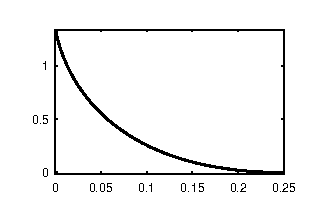
\includegraphics[width=5cm]{PDF/Logistic_var}}
\caption{Entropy functional  $\phi$ derived from the  logistic distribution with
  $T_1(x) = x^2$.}
\label{fig:Entropy-logistic-var}
\end{figure}


% ---------- Logistic first order

\subsection{The logistic distribution and (partial) first-order moment(s)}
\label{subsec:LogisticFirstOrder}

Since $f_X$ and $T(x) = x$ do no share the same symmetries, one cannot interpret
the logistic  distribution as  a maximum entropy  constraint by the  first order
moment.   However, constraining  the  partial means  over  $\X_\pm =  \Rset_\pm$
allows  such  an  interpretation,  using  then multiform  entropies,  while  the
alternative  is to  relax the  concavity  property of  the entropy.  To be  more
precise, one chooses either functions $T_{-,1}(x) = $ and $T_{+,1}$, or function
$T_1$ under the form
%
\[
T_{\pm,1}(x) = x, \quad x \in \X_\pm = \Rset_\pm \qquad \mbox{or} \qquad T_1(x)
= x, \quad x \in \X = \Rset
\]
%
Over each set $\X_\pm$ the  inverse distribution writes $f_{X,\pm}^{-1}(y) = \pm
\, s \, \argtanh \sqrt{1-4 s y}$, leading to
%
\[
\phi'_\pm(y) = \lambda_0 + 2 s \, \lambda_{\pm,1} \argtanh \sqrt{1-4 s y} \qquad
\mbox{or} \qquad \widetilde{\phi}'_\pm(y) = \lambda_0 \pm 2 s \, \lambda_1
\argtanh \sqrt{1-4 s y}
\]
%
where the sign is absorbed on $\lambda_{\pm,1}$. A judicious choice is then
%
\[
\lambda_0 = 0 \qquad \mbox{and} \qquad \lambda_{\pm,1} = -1 \qquad \mbox{or}
\qquad \lambda_1 = -1
\]
%
leading either to the (convex) uniform function $\phi$,
\[
\phi(y) = \left( \frac12 \, \sqrt{1 - 4 s y} - 2 s y \argtanh \sqrt{1 - 4 s y}
\right) \un_{\left[ 0 \, ; \, \frac{1}{4 s} \right]}(y)
\]
%
or to the multiform function $\phi$ with branches $\widetilde{\phi}_\pm$,
\[
\widetilde{\phi}_\pm(y) = \pm \left( \frac12 \, \sqrt{1 - 4 s y} - 2 s y \argtanh
\sqrt{1 - 4 s y} \right) \un_{\left[ 0 \, ; \, \frac{1}{4 s} \right]}(y)
\]
%
Function $\phi$ is represented figure \ref{fig:Entropy-logistic-moy}  for $s =
1$.
%
\begin{figure}[htbp]
\centerline{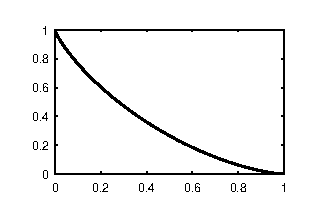
\includegraphics[width=5cm]{PDF/Logistic_moy}}
\caption{Entropy functionals $\phi$ derived  from the logistic distribution with
  either partial moments $T_{\pm,1}(x) = x \un_{\Rset_\pm}(x)$, or global moment
  $T_1(x) = x$ (here $\widetilde{\phi}_\pm = \pm \phi$).}
\label{fig:Entropy-logistic-moy}
\end{figure}

The choice  of $\lambda_{\pm,1}$ allows in  a sense to respect  the symmetries of
the distribution, allowing thus to recover a classical $\phi$-entropy.


% ---------- Gamma first order

\subsection{The gamma distribution and (partial) first-order moment(s)}
\label{subsec:GammaFirstOrder}

As a very special case, consider here this distribution, expressed as
%
\[
f_X(x) = \frac{\beta^\alpha x^{\alpha-1} \exp(-\beta x)}{\Gamma(\alpha)} \qquad
\mbox{on} \qquad \X = \Rset_+.
\]
%
Let  us concentrate  on the  case $\alpha  > 1$  for which  the  distribution is
non-monotonous,   unimodal,    where   the   mode    is   located   at    $x   =
\frac{\alpha-1}{\beta}$    and   $f_X(\Rset_+)    =   \left[    0   \,    ;   \,
  \frac{\beta}{\Gamma(\alpha)}   \left(  \frac{\alpha-1}{e}  \right)^{\alpha-1}
\right]$.  Thus, here again it cannot  be viewed as a maximum entropy constraint
by the first order moment. Here, we  can again interpret it as a maximum entropy
constrained by the partial means
%
\[
T_{0,1}(x) = x \quad \mbox{over} \quad \X_0 = \left[ 0 \, ; \,
\frac{\alpha-1}{\beta} \right), \quad \mbox{and} \quad T_{-1,1}(x) = x \quad
\mbox{over} \quad \X_{-1} = \left[\frac{\alpha-1}{\beta} \, ; \: + \infty
\right).
\]
%
or as an extremal entropy constrainted by the mean
%
\[
T_1(x) = x \quad \mbox{over} \quad \X = \Rset_+
\]
%
%
Inverting $y = f_X(x)$ leads to the equation
%
\[
\frac{\beta x}{1-\alpha} \exp\left(\frac{\beta x}{1-\alpha}\right) = -
\frac{1}{\alpha-1} \left( \frac{\Gamma(\alpha) y}{\beta}
\right)^{\frac{1}{\alpha-1}}
\]
%
to be solved. As expected, this  equation has two solutions. These solutions can
be expressed via  the multivalued Lambert-W function $\W$ defined  by $z = \W(z)
\exp(\W(z))$, leading to
%
\[
\phi'_k(y) = \lambda_0 + \frac{\alpha-1}{\beta} \lambda_{k,1} \W_k \left( -
\frac{1}{\alpha-1} \left( \frac{\Gamma(\alpha) y}{\beta}
\right)^{\frac{1}{\alpha-1}} \right), \qquad y \in \left[ 0 \, ; \,
\frac{\beta}{\Gamma(\alpha)} \left( \frac{\alpha-1}{e}\right)^{\alpha-1} \right],
\]
%
and  similarely  for $\widetilde{\phi}_k$,  where  $\lambda_{k,1} =  \lambda_1$,
where  $k$ denotes the  branch of  the Lambert-W  function.  $k  = 0$  gives the
principal branch and here it is related  to the entropy part on $\X_0$, while $k
= -1$ gives the secondary branch, related to $\X_{-1}$ here. To design a concave
entropy,  to respect the  sense of  variation imposed  on $\phi_k'(y)$,  one can
choose
%
\[
\lambda_0 = 0 \qquad \mbox{and } \: \lambda_{k,1} \: \mbox{ such that} \qquad
(-1)^{k+1} \, \lambda_{k,1} > 0
\]
%
Indeed, there is  no judicious choice allowing to  compensate for the asymmetry
of $f_X$  and then  allowing the  definition of an  uniform function  $\phi$. In
general,  there is  no  closed form  for  $\phi_k(y)$. However,  when $\alpha  =
2,\ldots$ is  integer\footnote{Note that  in this case,  for $\beta  = \frac12$,
  $f_X$ is  a chi-squared distribution with  $2 \alpha$ degrees  of freedom}, it
can be checked that
%
\[
\phi_k(y) = \frac{\displaystyle (-1)^{k+1} \, \overline{\lambda}_{k,1} \: y
\sum_{m=0}^\alpha \mu_m \left[\W_k\left(- \frac{1}{\alpha-1} \left(
\frac{\Gamma(\alpha) y}{\beta} \right)^{\frac{1}{\alpha-1}} \right)
\right]^m}{\left[\W_k\left(- \frac{1}{\alpha-1} \left( \frac{\Gamma(\alpha)
y}{\beta} \right)^{\frac{1}{\alpha-1}} \right) \right]^{\alpha-1}} \, + \, c_k
\]
%
where
%
\[
\mu_m = \frac{(-1)^{\alpha-m} \, \Gamma(\alpha)}{\Gamma(m+1) \,
(\alpha-1)^{\alpha-m}}, \quad m = 0, \ldots, \alpha-1, \quad \mbox{and} \quad
\mu_\alpha = 1
\]
%
% Voir avec des pochamer
$c_k$ is  an integration constant and  the multiplicative factor  is absorbed in
the  strictly  positive  $\overline{\lambda}_{k,1}$. $\X_{-1}$  being  unbounded,
$c_{-1}$ is  chosen to be zero and  $c_0$ can be chosen  such that $\phi_k\left(
  \frac{\beta}{\Gamma(\alpha)}   \left(   \frac{\alpha-1}{e}  \right)^{\alpha-1}
\right)$  coincide  for  instance. The same algebra leads to the same expression for the $\widetilde{\phi}_k$, except that $(-1)^{k+1} \lambda_{k,1}$ are replaced by a unique $\lambda_1$.

The  multivalued   function  $\phi$  in  the  concave   context  is  represented
figure~\ref{fig:Entropy-gamma-moy} for $\beta  = 3$, $\alpha = 2$  and $\alpha =
5$, and with the choices  $\overline{\lambda}_{k,1} = 1$ (for the other context,
with $\overline{\lambda}_1 = -1$, $\widetilde{\phi}_k = (-1)^k \phi_k$.)
% = - \frac{2 \beta}{e}$.
%
\begin{figure}[htbp]
\centerline{
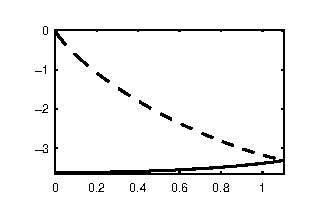
\includegraphics[width=5cm]{PDF/Gamma_2_moy} \hspace{2mm}
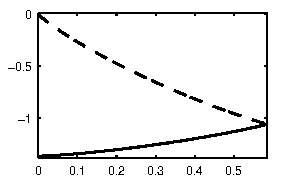
\includegraphics[width=5cm]{PDF/Gamma_5_moy}}
%
\caption{Multiform entropy functional $\phi$ derived from the gamma distribution
  with $\beta = 3$,  $T_{k,1}(x) = x \un_{\X_k}(x)$, $k \in \{0  , -1 \}$ (solid
  line $\phi_0$ and dashed line $\phi_{-1}$). Left: $\alpha = 2$; Right: $\alpha
  = 5$.}
\label{fig:Entropy-gamma-moy}
\end{figure}
%
% (this choice is made to see each branch);
% \lambda_{0,1}   >  0 mais attention, phi_k' = - (a-1)/b W_k(-...)
% \lambda_{-1,1}  <   0


% ---------- Gamma second order

\subsection{The gamma distribution and (partial) second-order moment(s)}
\label{subsec:GammaSecondOrder}

Now, we consider as constraints the ``partial'' second-order moments
%
\[
T_{0,1}(x) = x^2 \quad \mbox{over} \quad \X_0 = \left[ 0 \, ; \,
\frac{\alpha-1}{\beta} \right), \quad \mbox{and} \quad T_{-1,1}(x) = x^2 \quad
\mbox{over} \quad \X_{-1} = \left[\frac{\alpha-1}{\beta} \, ; \: + \infty
\right)
\]
%
The same approach than in the previous case leads to
%
\[
\phi'_k(y) = \lambda_0 + \left(\frac{\alpha-1}{\beta}\right)^2 \lambda_{k,1}
\left[ \W_k \left( - \frac{1}{\alpha-1} \left( \frac{\Gamma(\alpha) y}{\beta}
\right)^{\frac{1}{\alpha-1}} \right) \right]^2, \qquad y \in \left[ 0 \, ; \,
\frac{\beta}{\Gamma(\alpha)} \left( \frac{\alpha-1}{e}\right)^{\alpha-1} \right]
\]
%
To respect the sense of variation imposed on $\phi_k'(y)$, one can choose again
%
\[
\lambda_0 = 0 \qquad \mbox{and } \: \lambda_{k,1} \: \mbox{ such that} \qquad
(-1)^{k+1} \, \lambda_{k,1} > 0
\]
%
and when $\alpha$ is integer ($\alpha \ge 2$), it can be checked that
%
\[
\phi_k(y) = \frac{\displaystyle (-1)^{k+1} \, \overline{\lambda}_{k,1} \: y
\sum_{m=0}^{\alpha+1} \mu_m \left[\W_k\left(- \frac{1}{\alpha-1} \left(
\frac{\Gamma(\alpha) y}{\beta} \right)^{\frac{1}{\alpha-1}} \right)
\right]^m}{\left[\W_k\left(- \frac{1}{\alpha-1} \left( \frac{\Gamma(\alpha)
y}{\beta} \right)^{\frac{1}{\alpha-1}} \right) \right]^{\alpha-1}} \, + \, c_k
\]
%
where
%
\[
\mu_m = \frac{2 \, (-1)^{\alpha-m+1} \, \Gamma(\alpha+1)}{\Gamma(m+1) \,
(\alpha-1)^{\alpha-m+1}}, \quad m = 0, \ldots, \alpha, \quad \mbox{and} \quad
\mu_{\alpha+1} = 1
\]
%
% Voir avec des pochamer
and $c_k$ is  an integration constant and the  multiplicative factor is absorbed
in the strictly positive  $\overline{\lambda}_{k,1}$. Again $c_{-1}$ is chosen to
be    zero    and   $c_0$    can    be    chosen    such   that    $\phi_k\left(
  \frac{\beta}{\Gamma(\alpha)}   \left(   \frac{\alpha-1}{e}  \right)^{\alpha-1}
\right)$    coincide.      This    multivalued    function     is    represented
figure~\ref{fig:Entropy-gamma-var} for $\beta  = 3$, $\alpha = 5$  and $\alpha =
10$, and with the choices $\overline{\lambda}_{k,1} = 1$
% = - \frac{2 \beta}{e}$.
%
\begin{figure}[htbp]
\centerline{
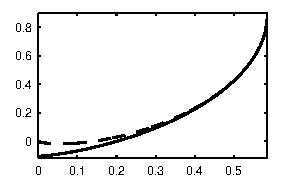
\includegraphics[width=5cm]{PDF/Gamma_5_var} \hspace{2mm}
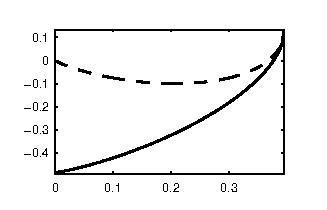
\includegraphics[width=5cm]{PDF/Gamma_10_var}}
%
\caption{Multiform entropy functional $\phi$ derived from the gamma distribution
  with $\beta = 3$, $T_{k,1}(x) = x^2 \un_{\X_k}(x)$, $k \in \{0 , -1 \}$ (solid
  line $\phi_0$ and dashed line $\phi_{-1}$). Left: $\alpha = 5$; Right: $\alpha
  = 10$.}
\label{fig:Entropy-gamma-var}
\end{figure}

Here again,  the approach  with a global  constraint $T_1(x)  = x^2$ over  $\X =
\Rset_+$,  with  the  choice  $\overline{\lambda}_1  = -  1$,  leads  simply  to
$\widetilde{\phi}_k = (-1)^k \phi_k$.
% (this choice is made to see each branch);
% \lambda_{0,1}   >  0 mais attention, phi_k' = - (a-1)/b W_k(-...)
% \lambda_{-1,1}  <   0


% ---------- Arcsine second order

\subsection{The arcsine distribution and second-order moment}
\label{subsec:ArcsineSecondOrder}

The arcsine distribution is a special case of the beta distribution with $\alpha
= \beta  = \frac12$. We  consider here the  centered and scaled version  of this
distribution which writes
%
\[
f_X(x) = \frac{1}{\pi \sqrt{2 \, \sigma^2 - x^2}} \qquad \mbox{on} \qquad \X =
(-\sigma \sqrt2 \, ; \, \sigma \sqrt2).
\]
%
The inverse  distributions $f_{X,\pm}^{-1}$ on $\X_-  = (-\sigma \sqrt2  \, ; \,
0)$ and $X_+ = [0 \, ; \, \sigma \sqrt2)$ write then
%
\[
f_{X,\pm}^{-1}(y) = \pm \frac{\sqrt{2 \pi^2 \sigma^2 y^2 - 1}}{\pi y}, \qquad y
\ge \frac{1}{\pi \sigma \sqrt2}
\]
%
When the second order moment $T_1(x) = x^2$ is constrainted, one obtains
%
\[
\phi'(y) = \lambda_0 + \lambda_1 \left( 2 \sigma^2 - \frac{1}{\pi^2 y^2} \right)
\]
%
With the special choice
%
\[
\lambda_0 = 0 \qquad \mbox{and} \qquad \lambda_1 = 1
\]
%
the entropy functional is then
%
\[
\phi(y) = 2 \sigma^2 y +\frac{1}{\pi^2 y} \qquad y \ge \frac{1}{\pi \sigma \sqrt2}
\]
%
which is represented figure~\ref{fig:Entropy-arcsin-var}
%
\begin{figure}[htbp]
\centerline{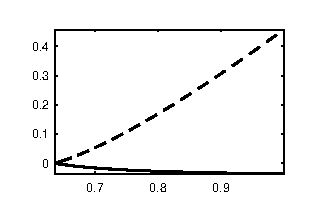
\includegraphics[width=5cm]{PDF/Arcsine_var}}
%
\caption{Entropy functional $\phi$ derived  from the centered and scaled arcsine
  distribution with constraints $T_1 = x^2$.}
\label{fig:Entropy-arcsin-var}
\end{figure}
%

% %-----------

% %
% \[
% T_{-,1}(x) = x^2 \quad \mbox{over} \quad \X_- = \left( 0 \, ; \, \frac12 \right),
% \quad \mbox{and} \quad T_{+,1}(x) = x^2 \quad \mbox{over} \quad \X_+ =
% \left[\frac12 \, ; \: 1 \right).
% \]
% %
% one obtains
% %
% \[
% \phi_{\pm}'(y) = \lambda_0 + \lambda_{\pm,1} \left( 1 - \frac{2}{\pi^2 y^2} \pm
% \frac{\sqrt{\pi^2 y^2-4}}{\pi y} \right)
% \]
% %
% The same choice
% %
% \[
% \lambda_0 = 0 \qquad \mbox{and } \qquad \lambda_{\pm,1} = \pm 1
% \]
% %
% leads to
% %
% \[
% \phi_\pm(y) = \frac{1}{\pi} \sqrt{\pi^2 y^2 - 4} + \frac{2}{\pi} \arctan \left(
% \frac{2}{\sqrt{\pi^2 y^2 - 4}} \right) \pm \left( y + \frac{2}{\pi^2 y} \right)
% + c_\pm
% \]
% %
% which  is represented  figure~\ref{fig:Entropy-arcsin-var} with  the integration
% constants chosen as $c_\pm = \mp \frac{3}{\pi} - 1$.
% %
% \begin{figure}[htbp]
% \centerline{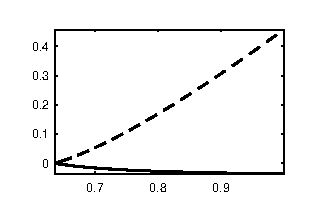
\includegraphics[width=5cm]{PDF/Arcsine_var}}
% %
% \caption{Multiform   entropy  functional   $\phi$  derived   from   the  arcsine
%   distribution  with constraints  $T_{\pm,1}  = x^2$:  solid  line $\phi_-$  and
%   dashed line $\phi_+$).}
% \label{fig:Entropy-arcsin-var}
% \end{figure}
%

% ---------- Arcsine first order

\subsection{The arcsine distribution and (partial) first-order moment(s)}
\label{subsec:ArcsineFirstOrder}

We consider  again the centered and  scaled version of  the arcsine distribution
with  first order  moment. Since  it does  not shar  the sense  of  variation of
$T_1(x) = x$, either  we turn out to consider it as  an extremal distribution of
an entropy that is not concave, or  as a maximum entropy when constraints are of
the type
%
\[
T_{\pm,1}(x) = x \quad \mbox{over} \quad \X_- = \left( -\sigma\sqrt2 \, ; \, 0
\right), \quad \mbox{and} \quad \X_+ = \left[0 \, ; \: \sigma \sqrt2 \right).
\]
%
now
%
\[
\phi_{\pm}'(y) = \lambda_0 + \lambda_{\pm,1} \frac{\sqrt{2 \pi^2 \sigma^2 y^2 -
1}}{\pi y}
\]
%
where the sign is absorbed  in the factors $\lambda_{\pm,1}$. A judicious choice
can be
%
\[
\lambda_0 = 0 \qquad \mbox{and } \qquad \lambda_{\pm,1} = 1
\]
%
leading then to the uniform function
%
\[
\phi(y) = \frac{1}{\pi} \sqrt{2 \pi^2 \sigma^2 y^2 - 1} + \frac{1}{\pi} \arctan
\left( \frac{1}{\sqrt{2 \pi^2 \sigma^2 y^2 - 1}} \right)
\]
%
This  function  is represented  figure~\ref{fig:Entropy-arcsin-moy}.
%with the integration constants chosen as $c_\pm = \mp \frac{2}{\pi} - 1$.
%
\begin{figure}[htbp]
\centerline{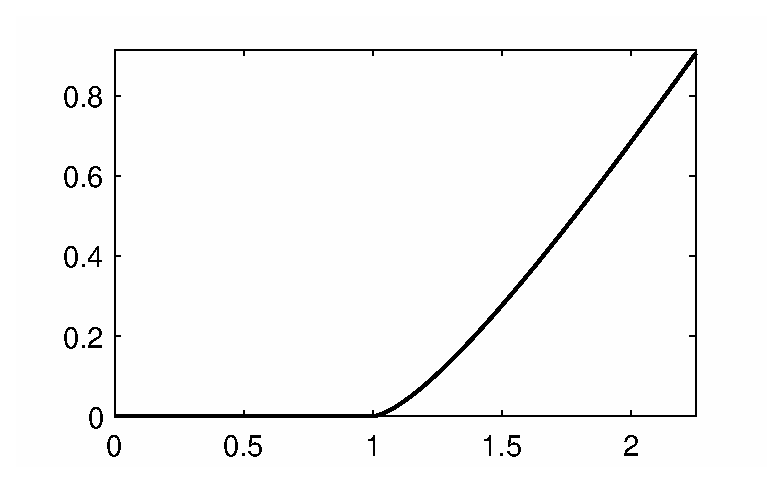
\includegraphics[width=5cm]{PDF/Arcsine_moy}}
%
\caption{Entropy  functional   $\phi$  derived   from   the  arcsine
  distribution with constraints $T_{\pm,1} =  x$.}
%: solid line $\phi_-$ and dashed  line $\phi_+$).}
\label{fig:Entropy-arcsin-moy}
\end{figure}

In the  approach with a constraint  impose over $\X$ but  relaxing the concavity
property of the entropy, one can easyly see we arrive at the multiform function
%
\[
\widetilde{\phi}_\pm(y) = \pm \phi(y)
\]
%
(with the choice $\lambda_1 = 1$).



%%%%%%%%%%%%%%%%%%%%%%%%%%%%%%%%%

\vspace{1cm}

\centerline{\underline{\hspace{10cm}}}

\vspace{1cm}


% ---------- q-Normal

%\subsection{Hyperbolic secant distribution and first-order moment}

Let us consider some specific cases. 
\begin{enumerate}
%
\item Let $f_{X}(x)$ be the hyperbolic nt distribution, with density
\[
f_{X}(x)=\frac12\text{sech}(\frac{\pi}{2}x)=\frac12\cosh^{-1}(\frac{\pi}{2}x).
\]
Obviously, $\frac{\pi}{2}x=\cosh(2y)=\phi'(y)$ with $T(x)=x$, $\lambda=\frac{\pi}{2}$,
and 
\[
\phi(y)=\sinh(2y).
\]
So doing, we obtain an hyperbolic sine entropy with the hyperbolic
secant distribution as the associated maximum entropy distribution.
\end{enumerate}

\end{document}
